\documentclass[border=2pt]{standalone}
\usepackage[T1]{fontenc}
\usepackage[tt=false]{libertine}
\usepackage[libertine]{newtxmath}
\usepackage[varqu]{zi4}
\usepackage{tikz}
\usetikzlibrary{positioning,arrows.meta,shapes.geometric,shapes.symbols,calc,fit,backgrounds}
% paper \textwidth (acmart sigconf) = 506.295pt; every variant is drawn to fit it at \small (8pt)
\newcommand{\tw}{506pt}

\begin{document}\small
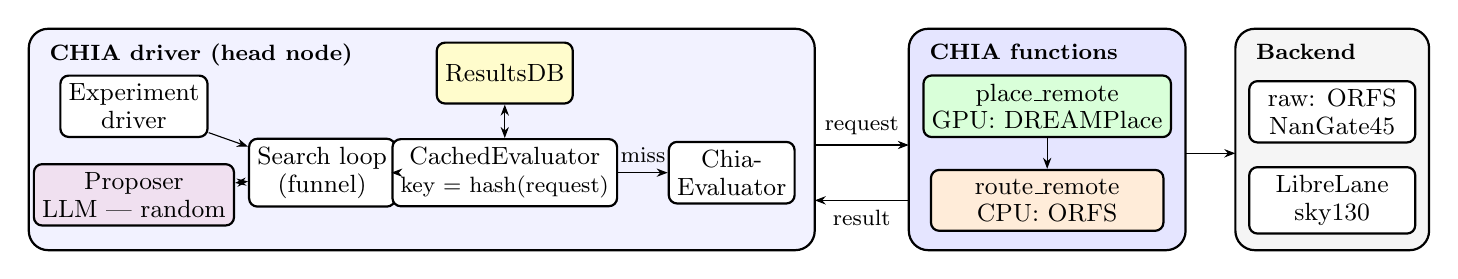
\begin{tikzpicture}[x=1pt,y=1pt,>={Stealth[length=4pt]},
  b/.style={draw,thick,rounded corners=3pt,align=center,inner sep=3pt,minimum height=22pt,fill=white,font=\small},
  lab/.style={font=\footnotesize,align=center},
  box/.style={rounded corners=7pt,thick,draw}]
% CHIA driver
\draw[box,fill=blue!5] (0,-40) rectangle (284,40);
\node[anchor=north west,font=\footnotesize\bfseries] at (4,38) {CHIA driver (head node)};
\node[b] (E) at (38,12) {Experiment\\[-1pt]driver};
\node[b,fill=violet!12] (P) at (38,-20) {Proposer\\[-1pt]LLM | random};
\node[b] (S) at (106,-12) {Search loop\\[-1pt](funnel)};
\node[b] (C) at (172,-12) {CachedEvaluator\\[-1pt]{\footnotesize key = hash(request)}};
\node[b,fill=yellow!20] (DB) at (172,24) {ResultsDB};
\node[b] (CE) at (254,-12) {Chia-\\[-1pt]Evaluator};
\draw[->] (E)--(S); \draw[<->] (P)--(S); \draw[->] (S)--(C); \draw[<->] (C)--(DB);
\draw[->] (C)--node[above,lab]{miss}(CE);
% Ray workers
\draw[box,fill=blue!10] (318,-40) rectangle (418,40);
\node[anchor=north west,font=\footnotesize\bfseries] at (322,38) {CHIA functions};
\node[b,fill=green!15,minimum width=84pt] (PL) at (368,12) {place\_remote\\[-1pt]GPU: DREAMPlace};
\node[b,fill=orange!15,minimum width=84pt] (RT) at (368,-22) {route\_remote\\[-1pt]CPU: ORFS};
\draw[->] (PL)--(RT);
% Backends
\draw[box,fill=black!4] (436,-40) rectangle (506,40);
\node[anchor=north west,font=\footnotesize\bfseries,align=left] at (440,38) {Backend};
\node[b,minimum width=60pt] (RAW) at (471,10) {raw: ORFS\\[-1pt]NanGate45};
\node[b,minimum width=60pt] (LL) at (471,-22) {LibreLane\\[-1pt]sky130};
\draw[->] (284,-2)--node[above,lab]{request}(318,-2); \draw[<-] (284,-22)--node[below,lab]{result}(318,-22);
\draw[->] (418,-5)--(436,-5);
\end{tikzpicture}
\end{document}
